\section{Leggi di Newton}
I $3$ principi della dinamica, o \textit{leggi di Newton}, sono le leggi classiche fondamentali per la descrizione del moto.

\paragraph{}
Il \textbf{\textit{principio di inerzia}} afferma che:

Un corpo in un sistema di riferimento inerziale (senza sollecitazioni) o è in \textit{quiete}, se non è sottoposto ad alcuna forza o le forze risultanti sono nulle, o gode di un moto di tipo \textit{rettilineo uniforme}, quindi con velocità costante e accelerazione uguale a zero.

\paragraph{}
Il \textbf{\textit{secondo principio}} afferma che:

Le cause dei moti (accelerazioni) sono dei vettori direttamente proporzionali alla forza risultante agente sull'oggetto e inversamente proporzionale alla sua massa.
\begin{equation}
    \vec{F} = m\vec{a}
    \label{secondaLeggeNewton}
\end{equation}

\paragraph{}
Il \textbf{\textit{terzo principio}}, o \textit{principio azione reazione}, afferma che:

Ogni qualvolta un corpo $A$ esercitata una forza sul corpo $B$, allora $B$ esercita una forza uguale di modulo e contraria su $A$. È intrinsecamente in ogni oggetto che possiede massa e non cambia in base alla gravità a cui è sottoposto.
\begin{equation}
    \vec{F}_{AB} = -\vec{F}_{BA}
    \label{terzaLeggeNewton}
\end{equation}

Altre leggi\dots
\paragraph{}

\textbf{\textit{Omogeneità del tempo}}: gli esperimenti non dipendono dal tempo, se tutti i fattori rimangono inalterati allora l’esperimento deve valere indistintamente dal tempo.


\textbf{\textit{Omogeneità dello spazio}}: gli esperimenti non dipendono dallo spazio o dal luogo geografico, se tutti i fattori rimangono inalterati l’esperimento rimane costante. 

\textbf{\textit{Esotropia dello spazio}}: ambiente in cui non ci sono direzioni privilegiate ad esempio si pensi ad un proiettile che viene sparato con un angolo di $45\gradi$ rispetto a Nord cade dopo tot metri, come lo stesso proiettile, a parità di condizioni iniziali, se venisse sparato verso sud.

\paragraph{}

\textbf{N.B} Secondo Newton spazio e tempo sono \textbf{assoluti}. Ora non è più vera questa affermazione in quanto nel 1905 con la teoria della \textbf{relatività ristretta}, lo spazio-tempo \textbf{dipende dall'osservatore}. La distanza spaziale o temporale risulta diversa se l'osservatore che la misura sia in moto o fermo rispetto all'oggetto osservato.

\newpage
\paragraph{Nomenclatura:}
\paragraph{}
\textit{Inerzia:} tendenza di un corpo ad opporre resistenza ad un cambio di moto. La massa, M, è la misura dell’inerzia di un corpo.

\textit{Peso:} dovuto alla forza gravitazionale che agisce su un corpo ed è uguale al prodotto della massa per l’accelerazione di gravità 

\begin{equation*}
    \vec{F} = m\veca
\end{equation*}

\textit{Forza:} vettore considerato come spinta o trazione e dato il secondo principio di Newton una forza può produrre un accelerazione. 

\textit{Forza risultante:} somma di tutte le forze agenti su un oggetto 


Il \textit{sistema di riferimento inerziale} è caratterizzato dalle seguenti condizioni: se un corpo non è sottoposto a forze o la somma delle forze risultanti è zero allora esso preserva lo stato di quiete o di moto rettilineo uniforme finché non viene perturbato. In altre parole si dice inerziale perché \textbf{l’accelerazione è pari a zero} per immaginarselo si pensi ad un oggetto nello spazio. 
Per molti esperimenti, soprattutto per quelli di breve durata, la terra può essere considerata approssimativamente un sistema di riferimento inerziale. 

\paragraph{Tipi di forze} 
\paragraph{}
\begin{align*}
\begin{tabular}{ l c r }
\toprule
Forza       &    \qquad    &   Tipo\\
\midrule
Attraente   &       \qquad    &   a distanza\\
Peso        &       \qquad    &   a distanza\\
Centripeta   &      \qquad     &   a distanza\\
Elettrica        &       \qquad    &   a distanza\\
Magnetica        &       \qquad    &   a distanza\\
Attrito        &       \qquad    &   a contatto\\
Galleggiamento &       \qquad    &   a contatto\\
Elastica &       \qquad    &   a contatto\\
\bottomrule
\end{tabular}
\end{align*}

\newpage
\subsection{Attrito}
Forza che si oppone al movimento o scorrimento di un un corpo su un'altro. Può essere di due tipi: \textit{statico} ($\mu_s$) se i due corpi sono fermi e uno o entrambi iniziano un movimento; \textit{dinamico} ($\mu_d$) se i due corpi sono già in movimento tra loro.

Normalmente
\begin{equation*}
  \mu_s > \mu_d
\end{equation*}

\subsection{Il piano inclnato}

\begin{figure}[H]
\centering
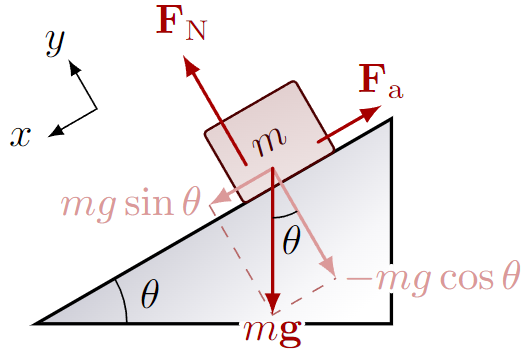
\includegraphics[width=0.45\textwidth]{image/attrito3.png}
\caption{Piano inclinato}
\label{img:pianoIncl}
\end{figure}


Il piano inclinato, un classico esempio per introdurre la scomposizione delle forza e l'attrito.

Come si vede nella Figura \ref{img:pianoIncl} stabiliamo innanzitutto un sistema di riferimento cartesiano lungo il piano inclinato. La forza peso, indicata con $ mg = \vec{F_p}$ è diretta verso il centro della terra, essa viene scomposta in due forze: una forza ortogonale al piano, indicata con $-mg\cos\theta = \vec{F_{py}}$, e una forza parallela al piano su cui poggia, indicata con $mg\sin\theta = \vec{F_{px}}$.

Per contrastare la forza peso ortogonale al piano troviamo la forza normale o reazione vincolare, indicata come $\vec{F_N} = \vec{R_V}$, che è  in direzione, verso e modulo opposto rispetto a $\vec{F_{py}}$. Se non ci fosse questa forza l'oggetto sprofonderebbe oppure sfonderebbe il sostegno sotto di esso. 

Si pensi ad un elefante su un tavolo da cucina, viene immediato a pensare che il povero tavolo venga sfondato dal pensate elefante. Infatti in questo esempio la reazione vincolare non è sufficiente per "sconfiggere" il peso dell'animale e dunque sorreggerlo.

L'ultima forza che rimane da analizzare è la forza di attrito statico, rivolta in verso e direzione opposta rispetto a $\vec{F_{px}}$ e rappresentata in figura \ref{img:pianoIncl} dalla forza $\vec{F_a}$.

\paragraph{Come trovare tutte le forze descritte in figura?}

Per il $2\gradi$ principio di Newton $(\vec{F} = m\vec{a})$ la forza peso è: 
\begin{equation*}
    \vec{F_p} = m\vec{g}\quad\bigg[\frac{N}{m}\bigg]
\end{equation*}
Dove m è la massa [Kg] dell'oggetto e $\vec{g}$ è la forza di gravità $\approx 9.81\mss$
\begin{equation*}
    \vec{F_{px}} = m\vec{g}\sin{\alpha}\quad \vec{F_{py}} = m\vec{g}\cos{\alpha}
\end{equation*}
\begin{equation*}
    \vec{F_a} = -\mu_s m\vec{g}\cos{\alpha}\quad \vec{R_v} = -m\vec{g}\sin{\alpha}
\end{equation*}



\subsection{La molla}
Una molla è un corpo capace di deformarsi a seconda delle forze che agiscono su di essa. Essa a seguito della deformazione genera una \textit{forza elastica}, che si oppone all'elongazione \footnote{Distanza rispetto alla sua posizione di equilibrio.} della molla che la induce a riacquisire la lunghezza originale.

Come si nota dalla figura \ref{img:molla} questa forza è direttamente proporzionale all'elongazione, e si esprime grazie alla legge sperimentale di Hooke, secondo la formula:

\begin{equation}
    \vec{F_e}  = -kx \qquad{con }\qquad x = L-L_0
    \label{ForzaElastica}
\end{equation}
%\clearpage  %newpage
Il segno meno nella legge di Hooke significa che la forza viene applicata in verso opposto all'elongazione: per gli allungamenti la forza di richiamo è negativa, mentre per le compressioni essa sarà positiva.

Altre formule:

\begin{itemize}
    \item costante elastica di molle in serie: $K_0 = \frac{k_1 +\dots{}+k_n}{k_1\cdot...\cdot K_n }$
    \item costante elastica di molle in parallelo: $K_0 = K_1+...+K_n$
    \item energia potenziale molla: $E_p = \frac{1}{2}K(\Delta x)^2$
    \item energia cinetica molla: $E_c = \frac{1}{2}m(\Delta v)^2$
\end{itemize}

\begin{figure}[H]%htbp H
\centering
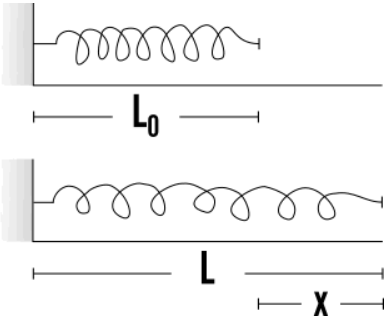
\includegraphics[width=0.45\textwidth]{image/molla}
\caption[Rappresentazio molla]{Rappresentazione elongazione molla}
\label{img:molla}
\end{figure}




\subsection{La Macchina di Atwood}

\begin{figure}[H]
    \centering
    \begin{tikzpicture}[scale=0.65]
    \centering
    % Mass 1
    \draw[thick] (1.49cm,0) -- ++(0,-5cm) node[draw=black,above=0.18cm,circle,fill=brown!70!black](cM){}
    node[draw=black,trapezium,rounded corners=1pt,fill=brown!70!black,text=white, minimum height=0.7cm](M){M};
    
    % Mass 2
    \draw[thick] (-1.49cm,0) -- ++(0,-3.5cm) node[draw=black,above=0.13cm,circle,fill=brown!70!black](cm){} node[draw=black,trapezium,rounded corners=1pt,fill=brown!70!black,text=white, minimum height=0.6cm](m){m};
    
    % Supporting structure
    \fill[pattern= north west lines,] (-2.5,2.41) rectangle (2.5,2.6);
    \draw(-2.5,2.41) -- (2.5,2.41);
    
    % Pulley
    \draw[fill = gray] (0,0) circle (1.5cm); % Big circle
    \draw[fill=lightgray] (0,0) circle (1.3cm); % Medium circle
    \draw[fill=white] (75:2.5) to[rounded corners=0.2cm] (0.2,-0.25) to[rounded corners=0.2cm] (-0.2,-0.25) -- (105:2.5) -- cycle;
    \draw[fill=darkgray] (0,0) circle (0.12cm); % Axle circle
    
    % Forces
    \draw [-latex,very thick,blue] (M.bottom side) -- ++(0,-1) node[midway,right]{$F_1$};
    \draw [-latex,very thick,black] (cM.north) -- ++(0,1)node[midway,right]{$T_1$};
    
    \draw [-latex,very thick,red] (m.bottom side) -- ++(0,-1)node[midway,left]{$F_2$};
    \draw [-latex,very thick,black] (cm.north) -- ++(0,1)node[midway,left]{$T_2$};
    
    \end{tikzpicture}
    \caption{Macchina di Atwood}
    \label{fig:atwood}
\end{figure}

La \textit{Macchina di Atwood}, raffigurata nella Figura \ref{fig:atwood}, è un apparato sperimentale ideato dal matematico inglese George Atwood per misurare l’accelerazione di gravità più facilmente e con una maggior grado di precisione di quanto non si potesse fare con il piano inclinato.

Intuitivamente si capisce che il corpo più pesante scenderà e farà ruotare la carrucola sollevando così il corpo più leggero.\\
In questo caso, per facilitare i calcoli, supponiamo che la corda e la carrucola non abbiano massa in modo tale che venga trasmessa tutta la forza senza dispersioni.

\newpage
\paragraph{}
Il concetto chiave da tenere in mente è che dovremo applicare il \textit{Secondo principio della Dinamica}: 

\begin{equation*}
    \vec{F}=m\veca
\end{equation*}

\paragraph{}

Per risolvere questi tipi di esercizi è fondamentale disegnare il \textit{Diagramma di corpo libero} già presente nell'immagine \ref{fig:atwood}, il quale rappresenta tutte le forze in gioco in un corpo massivo come ad esempio la forza peso, la tensione, la reazione vincolare, la forza di attrito\dots

Per ciascuno dei due corpi scriviamo l'equazione delle forze dettate dal \textit{Secondo principio della Dinamica}: 

$$
\begin{cases}

    M\vec{g} + T_1 = M\veca\\
    m\vec{g} + T_2 = m\veca
     
\end{cases}
$$
\begin{center}
 Dove: \qquad $M\vec{g} = F_1$ \quad ,  \quad $m\vec{g} = F_2$   
\end{center}

Poiché in entrambi i casi stiamo lavorando lungo un’unica direzione, possiamo riscrivere le precedenti equazioni specificando i segni delle grandezze coinvolte. Per il corpo M consideriamo un riferimento con verso delle coordinate crescenti rivolto verso il basso, per assecondare la forza di gravità. Per il corpo m invece prendiamo come verso delle coordinate crescenti quello rivolto verso l’alto in modo da assecondare la tensione della fune.

$$
\begin{cases}

    M\vec{g} - T_1 = M\veca\\
    -m\vec{g} + T_2 = m\veca
     
\end{cases}
$$
\begin{center}
 Dove: \qquad $M\vec{g} = F_1$ \quad ,  \quad $-m\vec{g} = F_2$   
\end{center}

Svolgendo i conti: 

\begin{equation*}
    M_1\vec{g} - mg\vec{g} = M\veca + m\veca \qquad \text{($T_1$ e $T_2$ si elidono)}
\end{equation*}

L'accelerazione di entrambi i corpi è:

\begin{equation}
    a = \frac{M-m}{M+m}\vec{g}
\end{equation}

La tensione della corda è:
\begin{equation}
    T = \frac{2 M m}{M+m}\vec{g}
\end{equation}


\newpage
\section{Moto Circolare}
Un corpo si dice che è in \textit{moto circolare} se esso si muove lungo una circonferenza di raggio $r$.

\paragraph{}
\textbf{Posizione angolare:}\\
Per descrivere questo moto conviene introdurre uno nuova grandezza fisica: \textit{la posizione angolare}. Figura \ref{fig:posizAng} \\
La \textit{posizione angolare} di un punto materiale è definita come l’angolo $\theta$ formato dal raggio passante per il punto con l’asse $x$.
La misura in radianti di un angolo $\theta$ è il rapporto fra la lunghezza l dell'arco tra l'asse $x$ e il punto e il raggio della circonferenza:

\begin{equation*}
    \theta_{rad} = \frac{l}{r} \qquad l=r\theta_{rad} \qquad 1\,rad = \frac{360\gradi}{2\pi}
\end{equation*} 

Nel SI, la posizione angolare, si misura in radianti al secondo: $\bigl[\frac{Rad}{s}\bigl]$

\begin{figure}[tb]
    \centering
    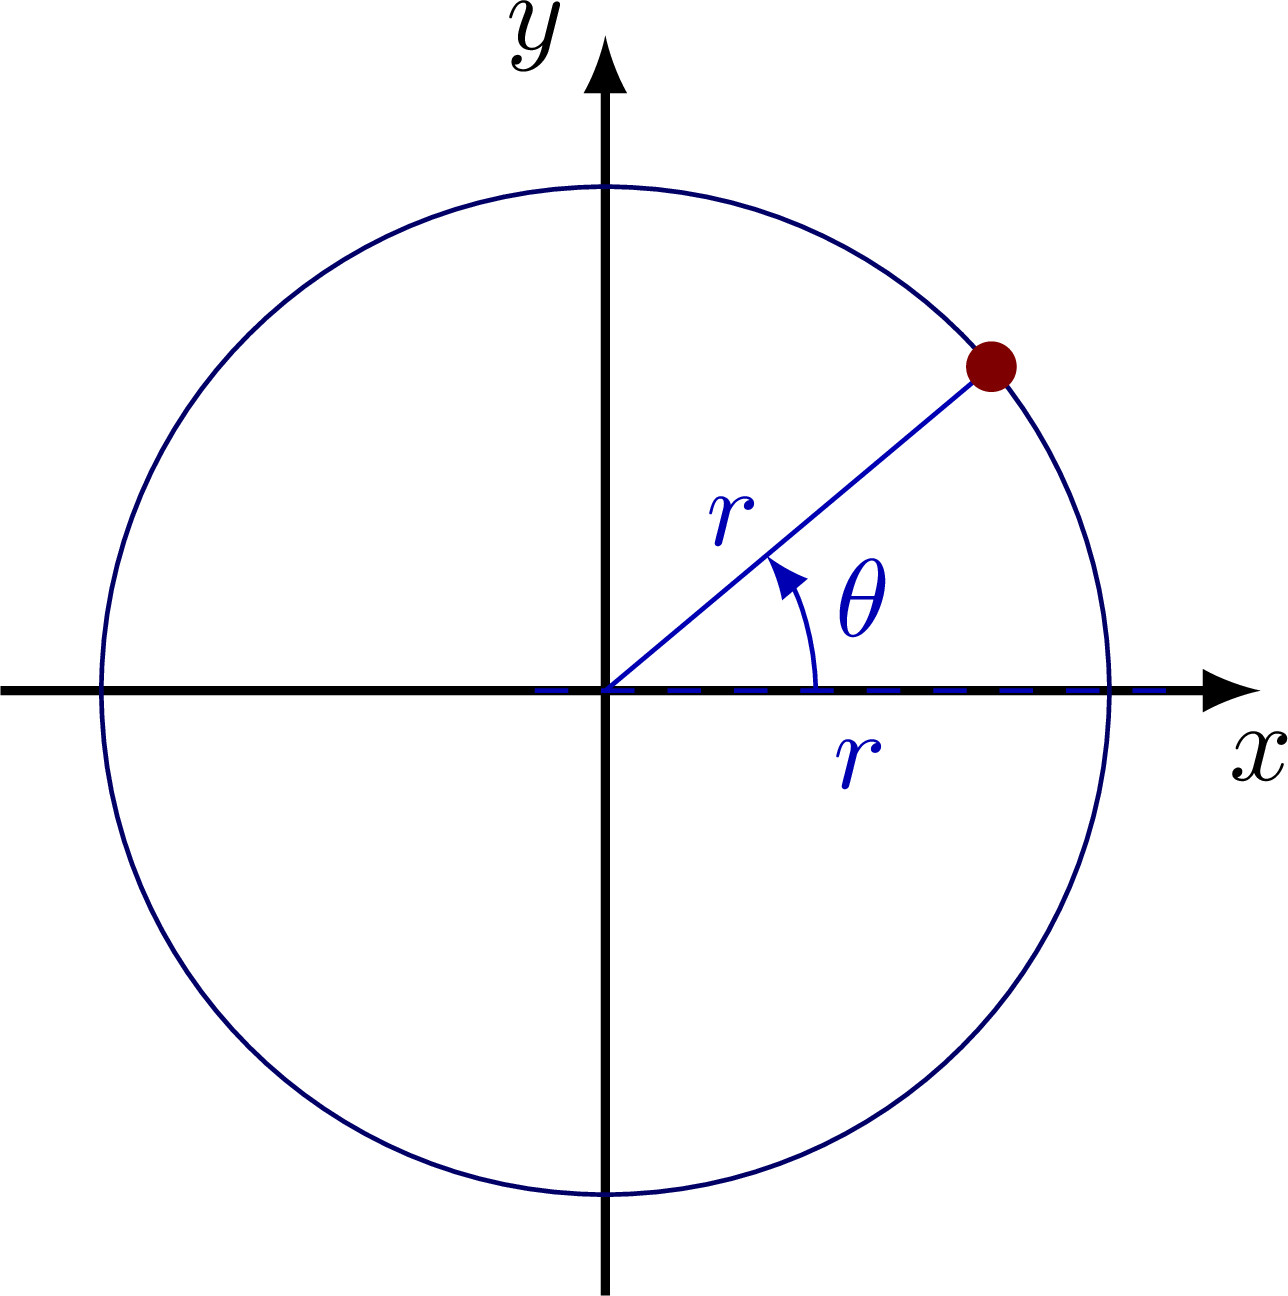
\includegraphics[width=0.45\textwidth]{image/posizioneAngolare.png}
    \caption{Posizione angolare}
    \label{fig:posizAng}
\end{figure}

\paragraph{}

\textbf{Velocità angolare:}\\

Al passare del tempo la posizione angolare del punto materiale che si muove su una traiettoria circolare cambia e dunque lo spostamento angolare $\Delta\theta$ del punto materiale è:

\begin{equation}
    \Delta\theta = \Delta_f - \Delta_i
\end{equation}

\begin{figure}
    \centering
    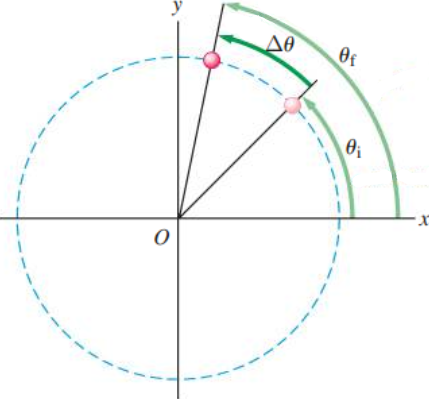
\includegraphics[width = 0.45\textwidth]{image/velocitaAng.png}
    \caption{Velocità angolare}
    \label{fig:velAng}
\end{figure}

Se dividiamo lo spostamento angolare per l’intervallo del tempo durante il quale avviene lo spostamento, otterremo la velocità angolare media:

\begin{equation}
    \omega_m = \frac{\Delta\theta}{\Delta t} \quad \biggl[\frac{rad}{s}\biggl]
\end{equation}

La velocità istantanea invece è: 

\begin{equation}
    \omega = \lim_{\Delta t \to 0} {\frac{\Delta\theta}{\Delta t}} \quad \biggl[\frac{rad}{s}\biggl]
\end{equation}

Questa definizione è analoga a quella della velocità istantanea lineare trattata in precedenza, si veda: \ref{velocitaLineare}

\paragraph{}
\textbf{Accelerazione tangenziale:}\\

Essendo che questo è un moto circolare uniforme allora l'accelerazione è nulla:

\begin{equation}
    \alpha = 0
\end{equation}


\paragraph{}
\textbf{Velocità tangenziale:}\\

Il modulo della velocità tangenziale $\vec{v}$ di un punto materiale è:

\begin{equation}
    v = \lim_{\Delta t \to 0}\frac{\Delta s }{\Delta t}  = \lim_{\Delta t \to 0}\frac{r\Delta \theta}{\Delta t} = \omega r \qquad \footnote{$\Delta s$ lung. del segmento che collega il punto al tempo $t_0$ con lo stesso punto al tempo $t_1$}
\end{equation}


\begin{figure}[H]
    \centering
    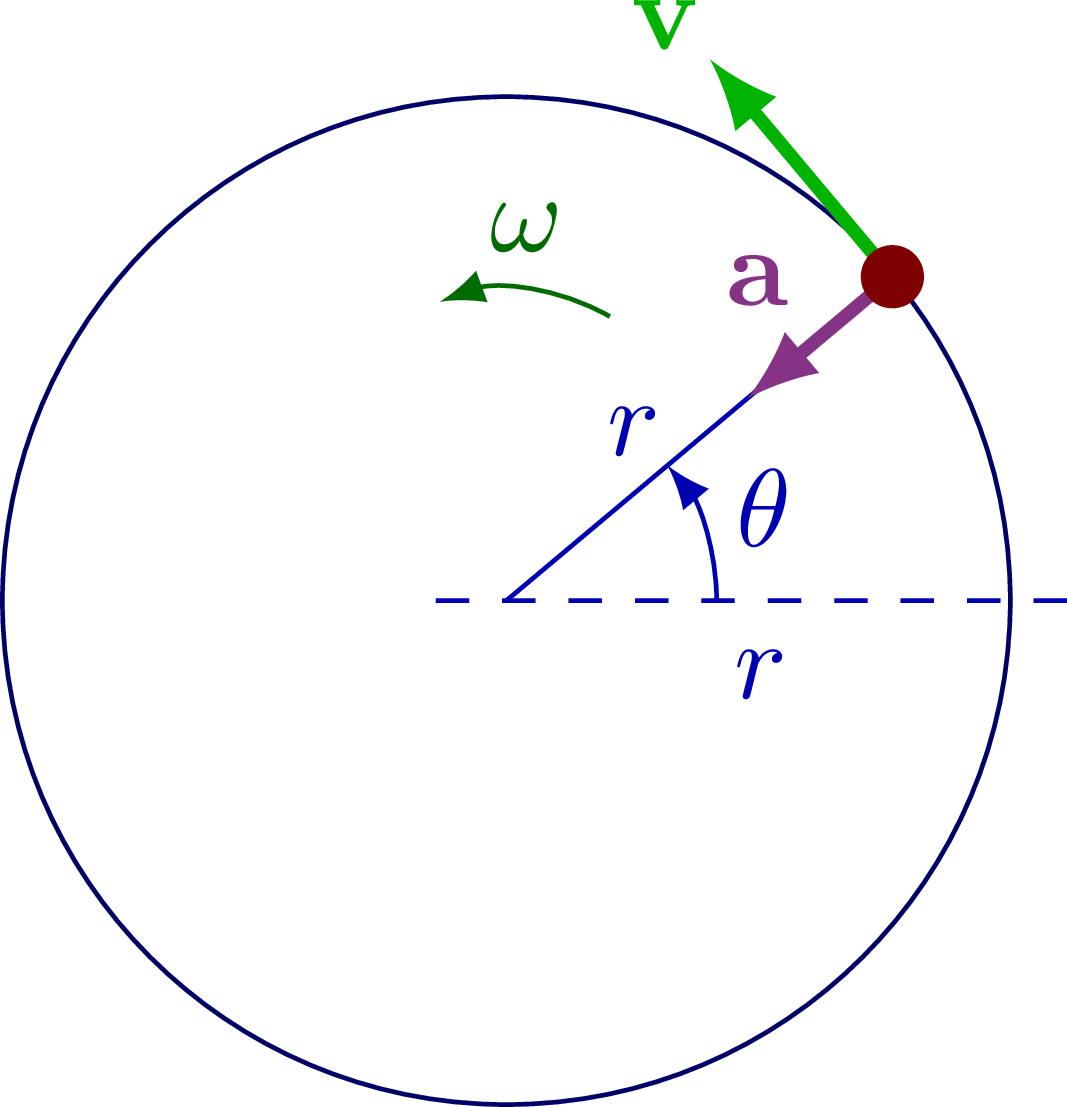
\includegraphics[width= 0.45 \textwidth]{image/motoCircUnif.png}
    \caption{Moto circolare uniforme}
    \label{fig:motoCircUnif}
\end{figure}

\paragraph{}
\textbf{Accelerazione centripeta:}\\

In particolare modo noi ci soffermeremo sul \textit{moto circolare uniforme},il quale ha velocità angolare e modulo delle velocità costanti, mentre la direzione varia essendo sottoposto ad un'accelerazione. Tale moto è un esempio di moto periodico, che si ripete ciclicamente nel tempo.
In un moto periodico $T$ è il tempo necessario per compiere un giro completo.

L'accelerazione costante viene chiamata \textit{accelerazione centripeta}, dal latino "diretta verso il centro". Figura \ref{fig:motoCircUnif}.

\paragraph{}
\textbf{Forza centrifuga}\\
\e una forza apparente applicata ad un oggetto massivo che gode di moto rotatorio. Questa è uguale in modulo e direzione opposta rispetto alla forza centripeta in un sistema inerziale, come in Figura \ref{fig:sistemaNonInerzialee}.

\def\R{2}      % disk radius
\def\t{0.1}    % disk thickness
\def\p{0.05}   % pole radius
\def\P{1.3}    % pole height
\def\r{0.24}   % mass radius
\def\L{0.7*\R} % rope length
\def\H{2.0}    % human height
\begin{figure}[H]
    \centering
    \begin{minipage}[c]{0.4\textwidth}
    
    \begin{tikzpicture}[scale = 1]
      \centering
      % PERSON
      \coordinate (H) at (0,\H);
      \draw[thick,line cap=round]
        (H)++(-165:0.3) to[out=-140,in=60]++ (-130:0.3)
        to[out=65,in=-90,looseness=1.0]++ (80:0.45) to[out=90,in=120,looseness=1.4]++ (20:0.2); % pony tail
      \draw[thick,fill=white] (H) circle (0.3);
      \draw[thick,line cap=round] (H)++(-140:0.3) to[out=80,in=-120,looseness=1.8]++ (40:0.6); % hair
      \draw[thick] (H)++(-90:0.3) coordinate (N) to[out=-95,in=95]++ (0,-0.40*\H) coordinate (P);
      \draw[thick,line cap=round] (N)++(-95:0.03) to[out=-60,in=95]++ (0.10*\H,-0.4*\H) coordinate (RH);
      \draw[thick,line cap=round] (N)++(-95:0.03) to[out=-120,in=90]++ (-0.08*\H,-0.4*\H);
      \draw[thick] (P) to[out=-70,in=95] (0.08*\H,0);
      \draw[thick] (P) to[out=-100,in=72] (-0.06*\H,0);
      
      % AXIS
      \node (A) at (0.38*\H,0.94*\H) {S};
      \draw[<->,line width=0.9]
        (A)++(0.25*\H,0.28*\H) node[left,scale=0.9] {$z$} --++ (0,-0.3*\H) coordinate (O) --++
             (0.3*\H,0) node[below right=-3.5,scale=0.9] {$y$};
      \draw[->,line width=0.9] (O) --++ (-120:0.25*\H) node[left=-2,scale=0.9] {$x$};
      
      % DISK
      \begin{scope}[shift={(0.5*\H+\R,0.3*\H)}]
        \coordinate (T) at (0,\r);
        \draw[disk] (-\R,0) --++ (0,-\t) arc(180:360:{\R} and {0.4*\R}) --++ (0,\t);
        \draw[disk] (0,0) ellipse({\R} and {0.4*\R});
        \rope {(T) --++ (\L,0) coordinate (M)};
        \draw[pole] (-\p,\P) --++ (0,-\P) arc(180:360:{\p} and {0.4*\p}) --++ (0,\P);
        \draw[pole] (0,\P) ellipse({\p} and {0.4*\p});
        \rope {(-1.4*\p,0.85*\r) arc(180:360:{1.4*\p} and {0.4*\p})}
        \rope {(-1.4*\p,1.00*\r) arc(180:360:{1.4*\p} and {0.4*\p})}
        \rope {(-1.4*\p,1.15*\r) arc(180:360:{1.4*\p} and {0.4*\p})}
        \draw[force] (M)++(150:1.1*\r) --++ (-0.5*\L,0) node[above=-1] {$\vb{T}$};
        \draw[avec] (M)++(210:1.1*\r) --++ (-0.5*\L,0) node[right=0,below=-1] {$\vb{a}$}; %_\mathrm{cm}
        \draw[mass] (M) circle(\r) node {$m$};
        \draw[->] (10:1.05*\R) arc(10:50:{1.05*\R} and {0.4*\R}) node[above left=-2] {$\omega$};
        \draw[vvec] (0,\P+0.014) --++ (0,0.7*\L) node[midway,left] {$\vb*\omega$};
      \end{scope}
      
    \end{tikzpicture}
    
    \caption{Sistema di riferimento inerziale}
    \label{fig:sistemaInerzialee}
    \end{minipage}
    \hspace{10mm}
    \begin{minipage}[c]{0.4\textwidth}
    \centering
    \begin{tikzpicture}[scale = 1]
  
      % DISK
      \coordinate (T) at (0,\r);
      \draw[disk] (-\R,0) --++ (0,-\t) arc(180:360:{\R} and {0.4*\R}) --++ (0,\t);
      \draw[disk] (0,0) ellipse({\R} and {0.4*\R});
      
      % PERSON
      \draw[thick,fill=white] (-0.35*\R,\H) circle (0.15*\H) coordinate (H);
      \draw[thick] (H)++(-90:0.15*\H) coordinate (N) to[out=-95,in=95]++ (0,-0.40*\H) coordinate (P);
      \draw[thick,line cap=round] (N)++(-95:0.03) to[out=-70,in=190]++ (0.34*\H,-0.20*\H);
      \draw[thick,line cap=round] (N)++(-95:0.03) to[out=-120,in=-80]++ (-0.17*\H,-0.12*\H) to[out=100,in=-100]++ (0.02*\H,0.25*\H);
      \draw[thick] (P) to[out=-70,in=95] ($(H)+(0.08*\H,-\H)$);
      \draw[thick] (P) to[out=-100,in=72] ($(H)+(-0.08*\H,-\H)$);
      
      % POLE + MASS
      \rope {(T) --++ (\L,0) coordinate (M)};
      \draw[pole] (-\p,\P) --++ (0,-\P) arc(180:360:{\p} and {0.4*\p}) --++ (0,\P);
      \draw[pole] (0,\P) ellipse({\p} and {0.4*\p});
      \rope {(-1.4*\p,0.85*\r) arc(180:360:{1.4*\p} and {0.4*\p})}
      \rope {(-1.4*\p,1.00*\r) arc(180:360:{1.4*\p} and {0.4*\p})}
      \rope {(-1.4*\p,1.15*\r) arc(180:360:{1.4*\p} and {0.4*\p})}
      \draw[force] (M)++(150:1.1*\r) --++ (-0.5*\L,0) node[above=-1] {$\vb{T}$};
      \draw[force] (M)++(30:1.1*\r) --++ (0.5*\L,0) node[above=0] {$\vb{F}_\mathrm{cf}$};
      \draw[mass] (M) circle(\r) node {$m$};
      
      % AXIS
      \node (A) at (57:0.88*\R) {S$'$};
      \draw[<->,line width=0.9]
        (A)++(0.25*\H,0.28*\H) node[left,scale=0.9] {$z'$} --++ (0,-0.3*\H) coordinate (O) --++
             (0.3*\H,0) node[below right=-3.5,scale=0.9] {$y'$};
      \draw[->,line width=0.9] (O) --++ (-120:0.25*\H) node[left=-2,scale=0.9] {$x'$};
      
    \end{tikzpicture}
    
    \caption{Sistema di riferimento non inerziale}
    \label{fig:sistemaNonInerzialee}
    \end{minipage}
\end{figure}


\paragraph{}
Di seguito vengono riportate tutte le formule utili.
\paragraph{}
\textbf{Legge oraria: }
\begin{equation}
    \theta = \theta_0 + \omega t
\end{equation}
\paragraph{}
Velocità tangenziale:
\begin{equation}
    v = \frac{2\pi r}{t} \qquad v = \omega r
\end{equation}

Velocità angolare:
\begin{equation}
    \omega = \frac{2\pi}{t}\qquad \omega = \frac{v}{r}
\end{equation}

Accelerazione angolare:
\begin{equation}
    \alpha = 0
\end{equation}

Accelerazione centripeta:
\begin{equation}
    a_c = \frac{v^2}{r}\qquad a_c=\omega^2r
    \label{AccelerazioneCentripeta}
\end{equation}

Forza centrifuga:
\begin{equation}
    F_c = \frac{mv^2}{r}\qquad F_c=m\omega^2r
\end{equation}

Frequenza:
\begin{equation}
    f = \frac{1}{T}
\end{equation}



\section{Moto Rotatorio}
Un corpo si dice che è in moto rotatorio se esso ruota su sé stesso.
Ogni punto di un corpo rigido rotante attorno ad un asse descrive una traiettoria circolare e pertanto segue le leggi del \textit{Moto circolare}.
Consideriamo una ruota di bicicletta, Figura \ref{fig:ruotaBici}, libera di ruotare al proprio asse, come mostrato in figura.

Quando la ruota gira, ogni suo punto si muove su una traiettoria circolare il cui centro è l’asse di rotazione.


\begin{figure}[H]
    \centering
    \def\R{1.6} % wheel rims inside
    \begin{tikzpicture}
      \def\ang{90} % angle
      \def\F{1.2}  % force size
      \coordinate (O) at (0,0);
      \coordinate (R) at (\ang:\R);
      \clip (-1.2*\Rr,-1.17*\Rr) rectangle (1.17*\Rr,1.54*\Rr);
      \wheel
      \draw[rvec] (O) -- (\ang:0.95*\R) node[midway,above=3,right=-1] {\contour{white}{$\vb{r}$}};
    \end{tikzpicture}
    \caption{Ruota di bicicletta}
    \label{fig:ruotaBici}
\end{figure}

\newpage

